MiniMax-H3 is a large diffusion model that turns a text prompt into a five-second video with synchronised audio. This post is about what you can do with very little: one consumer GPU, no training run, no cluster. We investigate how much faster such a model can be served under that constraint, and what the trade-offs look like when you get there. Everything below was measured on a single RTX 4090, with a single A100 used only to score videos. We measured where the time actually goes, tried a shelf of published acceleration ideas one by one, and then combined the ones that worked. The combination we now run finishes a request in 130 seconds where the baseline took 327 seconds, and we try to be honest about what that costs in output quality.

Everything below is measured on one frozen workload: a 1344$\times$768 video at 124 frames and 24 FPS with 32 kHz stereo audio, generated end to end from a prompt, with the same seed everywhere. Timings are the wall time from submitting the request to having the finished file on disk, which includes the continuous shuttling of model weights between main memory and the GPU. Quality is scored with VBench \citep{huang2024vbench}, a suite of video-quality metrics, and we always compare like for like: same hardware, same prompts, same seed, paired clip by clip.

\section{Choosing a baseline worth accelerating}

The first job was picking the serving stack to accelerate. We screened five ways of running the model on the same sixteen prompts: ComfyUI with the Turbo 4-step and 8-step distilled checkpoints \citep{comfyui}, SGLang \citep{zheng2024sglang} with the LightX2V 4-step adapter \citep{lightx2v}, SGLang with the Larry 8-step adapter, and a FastH3 variant with a different attention backend. Two candidates were much faster than everything else, and of those, SGLang with LightX2V was the one whose output we could not distinguish from the slow dense baseline on our metrics. That became the baseline for all later work.

\begin{quote}
\textbf{Box: What is LightX2V?} LightX2V \citep{lightx2v} is a \emph{distilled} version of MiniMax-H3 \citep{minimaxh3}. A distilled model is trained to copy the output of a slower teacher, and LightX2V copies the teacher so well that it needs only four denoising passes instead of the usual dozens. The catch is that the model is tuned to one exact computation recipe, so any change to the numerics, however small, moves it away from what it was trained for. This comes back later.
\end{quote}

Before optimising anything, we timed the pipeline stage by stage. Table~\ref{tab:stages} is the anatomy of one request. Almost all of the time sits in the denoising stage, and inside that stage most of the time is not arithmetic. Because the model does not fit on the card, its weights live in main memory and are copied to the GPU layer by layer on every single pass. That copying is the real cost centre, and it shapes everything that follows.

\begin{table}[ht]
\centering
\caption{Where one baseline request spends its 326.5 seconds (RTX 4090). ``Decode and save'' covers turning the internal representation into a video file with its audio track.}\label{tab:stages}
\begin{tabular}{lrl}
\toprule
Stage & Time (s) & What happens there\\
\midrule
Text encoding & 48.6 & The prompt becomes conditioning vectors\\
Denoising (4 passes) & 256.9 & The model runs; weights stream from RAM to GPU throughout\\
Decode and save & 19.0 & Latents become video and audio on disk\\
\bottomrule
\end{tabular}
\end{table}

\section{What we tried, one module at a time}

We then worked through the literature, one technique at a time, keeping everything else frozen. Each arm had to pass the same gates: real native kernels rather than fallbacks, strict memory headroom, and a paired quality check. Figure~\ref{fig:individual} summarises the speed outcomes, and Table~\ref{tab:modules} adds the quality notes.

\begin{figure}[ht]
\centering
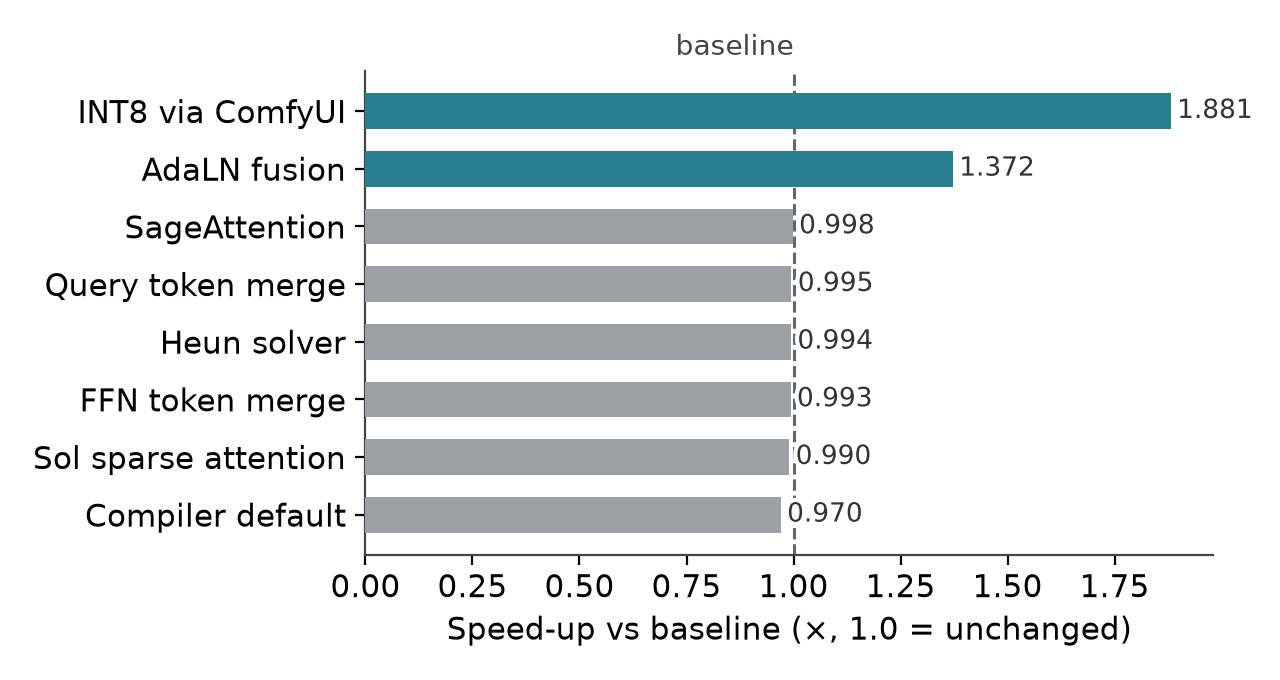
\includegraphics[width=0.85\linewidth]{assets/images/blog/miniacc/chart-individual-modules.png}
\caption{Speedup of each candidate run on its own, relative to the 1.0 baseline. Only the two techniques that reduce data movement beat the baseline.}\label{fig:individual}
\end{figure}

\begin{table}[ht]
\centering
\caption{Every module tested on its own. ``Quality'' is the paired VBench outcome against the baseline.}\label{tab:modules}
\begin{tabular}{llll}
\toprule
Module & Category & Speedup & Quality\\
\midrule
AdaLN fusion & kernel/memory & 1.372$\times$ & bitwise-identical outputs\\
INT8 weights (ComfyUI) & quantization & 1.881$\times$ & passed; single-run caveat\\
Compiler default & kernel & 0.970$\times$ & small changes\\
Sol & sparse attention & 0.990$\times$ & near-neutral; correctness gate failed\\
FFN token merge & token reduction & 0.993$\times$ & severe loss\\
Query merge & token reduction & 0.995$\times$ & severe loss ($-$24.7 overall)\\
Heun & solver & 0.994$\times$ & severe loss ($-$28.0 overall)\\
Cache-DiT & memory/cache & --- & never fit our memory floor\\
SageAttention & kernel & 0.998$\times$ & looked fine at 4 clips\\
\bottomrule
\end{tabular}
\end{table}

A few of these deserve a sentence each. AdaLN fusion precomputes small per-layer conditioning values once instead of recomputing them on every pass, and it was the cleanest win: the outputs were bit-for-bit identical to baseline while running 37\% faster. The INT8 weight quantiser from the ComfyUI ecosystem \citep{comfyui} stores the weights as 8-bit integers, halving the bytes that travel to the GPU, and it nearly doubled the speed. On the other side, both token-reduction methods \citep{bolya2023tome} and the higher-order solver \citep{hairer1993ode} destroyed quality, which is what you should expect once you understand the LightX2V box above: the model was distilled for one exact recipe, and these methods change the recipe. Cache-DiT \citep{cachedit} simply never fit in our memory budget.

\begin{quote}
\textbf{Box: What is Sol attention?} Sol \citep{li2026solattn} is a sparse-attention method. Attention normally compares every token with every other token, which is expensive at 37 thousand tokens \citep{dao2022flashattention}. Sol instead picks a small set of promising token pairs per head and only computes those, in our case about 13.5\% of all pairs, then adds a correction term for accuracy. Sparse attention is attractive on paper, but two things went wrong for us: the correction machinery cost more than the pairs it saved, and on real model inputs its numbers failed our correctness checks.
\end{quote}

\begin{quote}
\textbf{Box: What is SageAttention?} SageAttention \citep{zhang2025sageattention} keeps the attention pattern dense but does the score computation in 8-bit integer arithmetic instead of 16-bit floating point. Integer math is cheaper per operation, and SageAttention is a proper compiled kernel, not a simulation. On its own in our pipeline it changed nothing measurable, because attention is only about a sixth of the request time.
\end{quote}

\section{Putting the winners together}

The two clear winners attacked different costs. AdaLN removed per-layer conditioning work, and the 8-bit weights halved the weight traffic. Combining them was the natural next step, and it is also where the story gets interesting. Figure~\ref{fig:breakdown} shows what happened to the anatomy of a request.

\begin{figure}[ht]
\centering
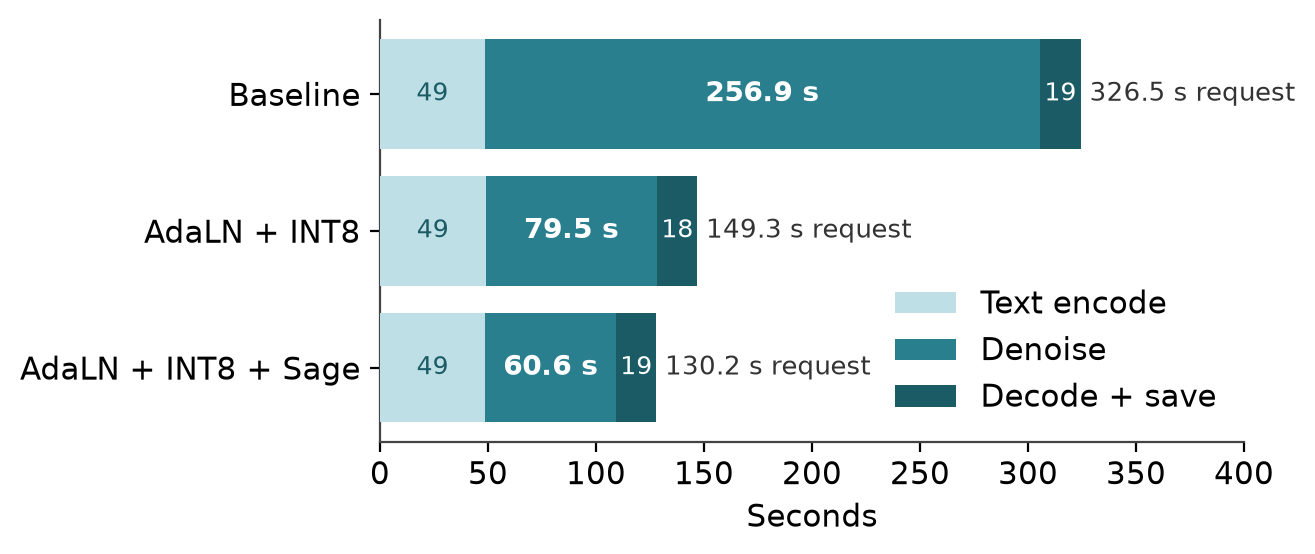
\includegraphics[width=0.9\linewidth]{assets/images/blog/miniacc/chart-time-breakdown.png}
\caption{Where a request spends its time as the techniques are layered on. The denoising stage shrinks from 257 to 61 seconds; text encoding and decoding are untouched.}\label{fig:breakdown}
\end{figure}

With the copying cost cut down, attention went from a sixth of the request to about a third of it. That is why SageAttention, which measured a flat 0.998$\times$ on its own, suddenly became useful. Its savings did not get bigger. Its share of the bill did. This is the most useful lesson of the whole exercise: on a memory-bound pipeline, compute optimisations are invisible until you remove the memory problem, and only then do they start to matter. Sol never got this rescue, because its operator is genuinely slower than the dense one it replaces. Making the pipeline cheaper does not fix a slow kernel.

\begin{figure}[ht]
\centering
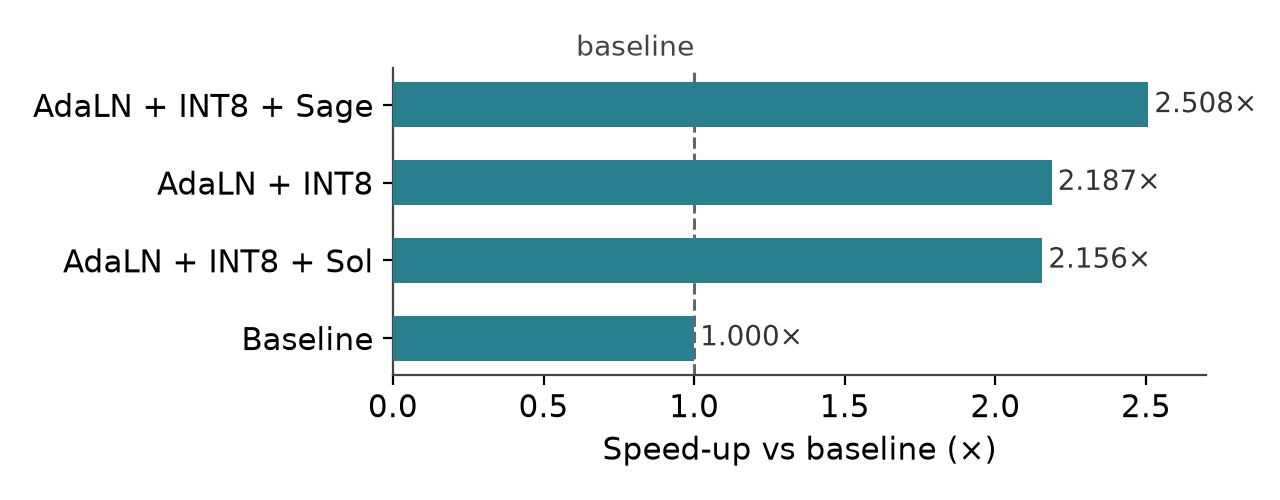
\includegraphics[width=0.85\linewidth]{assets/images/blog/miniacc/chart-integrated.png}
\caption{The integrated configurations against baseline. The final default includes SageAttention; the Sol variant is shown for completeness.}\label{fig:integrated}
\end{figure}

Figure~\ref{fig:integrated} shows the final speed numbers. AdaLN and the INT8 quantiser together give 2.19$\times$. Adding SageAttention on top reaches 2.51$\times$, our default configuration. Adding Sol instead gives 2.16$\times$.

\begin{figure}[ht]
\centering
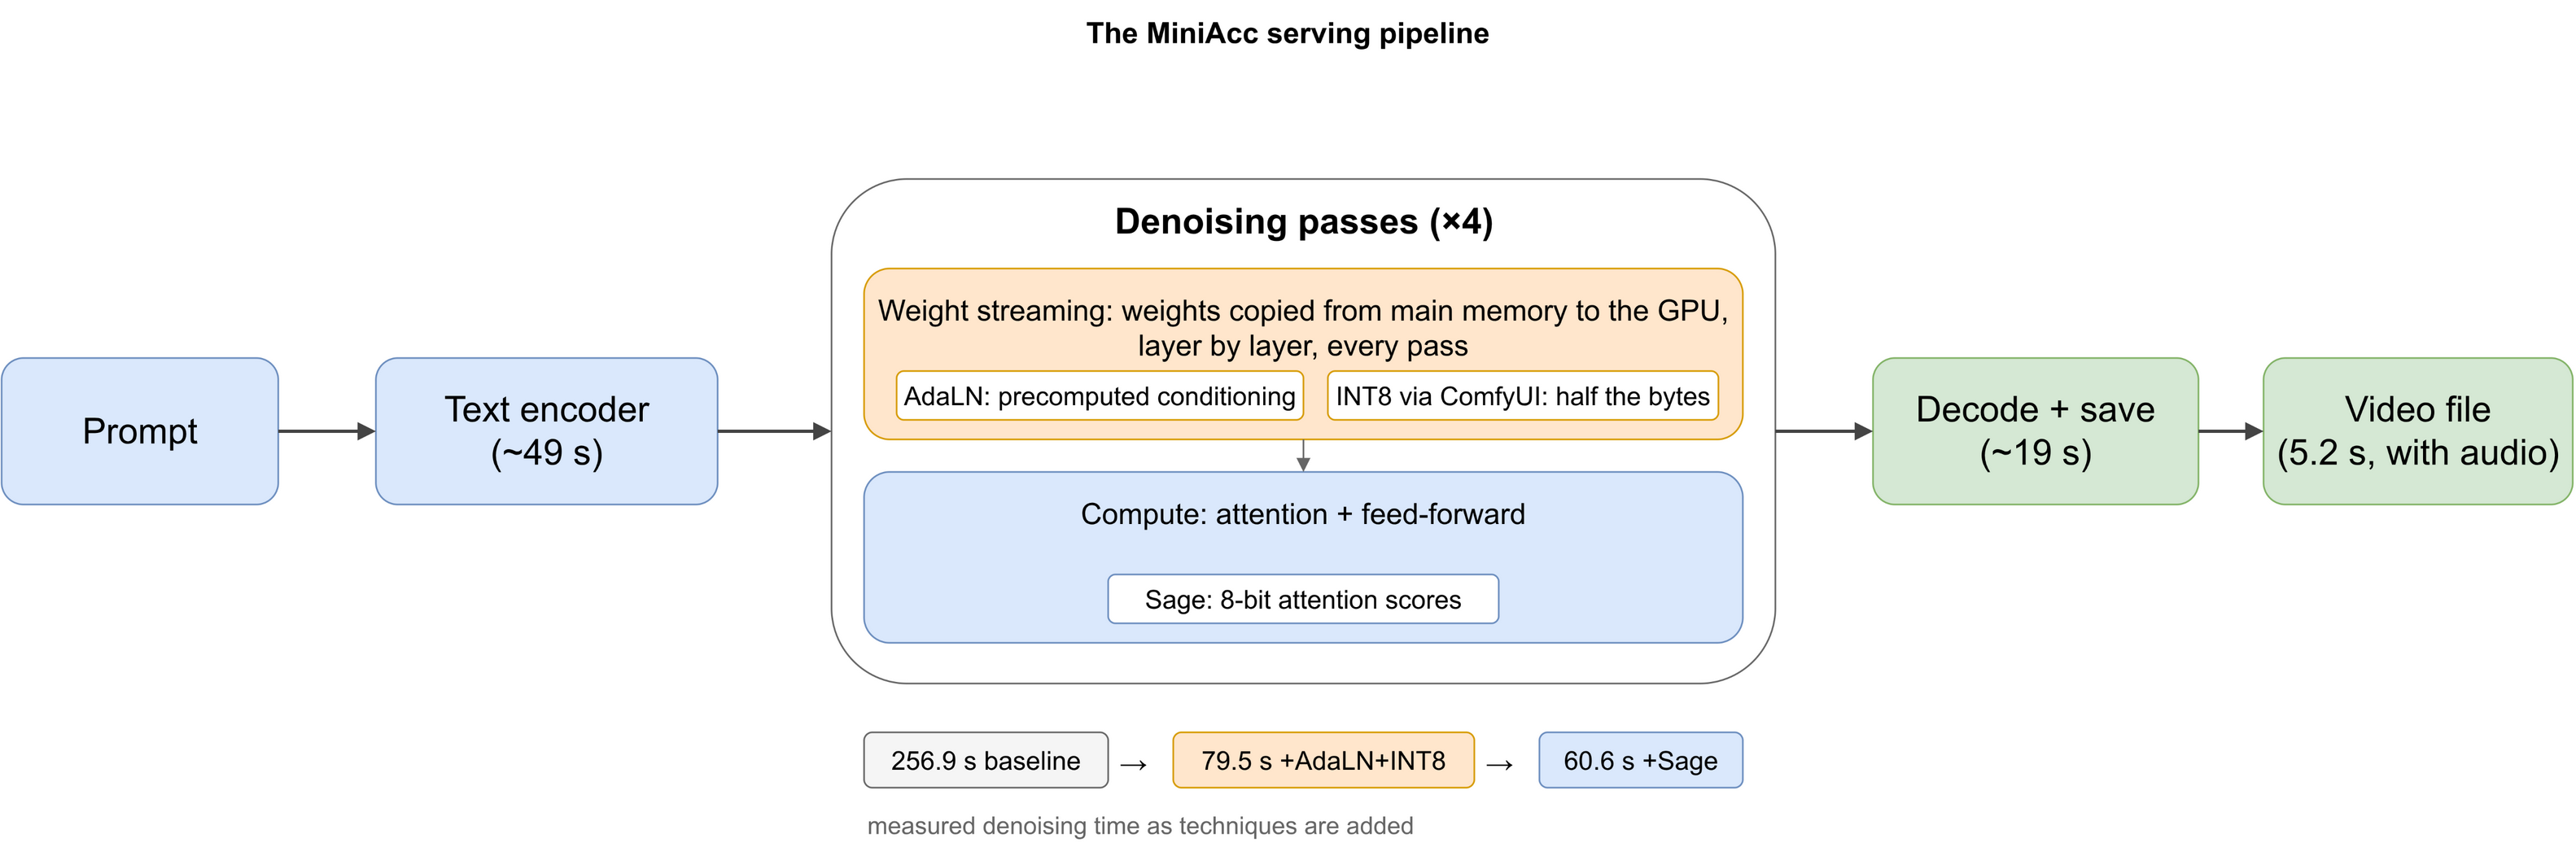
\includegraphics[width=\linewidth]{assets/images/blog/miniacc/pipeline-diagram.png}
\caption{The serving pipeline and where each technique acts. The warm lane is the bottleneck: weights are copied from main memory to the GPU on every denoising pass.}\label{fig:diagram}
\end{figure}

\section{Re-checking quality at scale: Sage and Sol}

Speed is only half the story, and this is where we had to be careful with ourselves. An early 4-clip check suggested SageAttention might even improve quality slightly. The 16-clip paired test said otherwise, and it was not close. Table~\ref{tab:quality16} shows the paired quality deltas against the Sage-free pipeline.

\begin{table}[ht]
\centering
\caption{Paired VBench quality deltas on the integrated pipeline (16 clips; negative is worse than the pipeline without that module).}\label{tab:quality16}
\begin{tabular}{lrr}
\toprule
Metric & Sage $\Delta$ & Sol $\Delta$\\
\midrule
Subject consistency & $+$0.14 & $+$0.63\\
Background consistency & $-$0.31 & $-$0.51\\
Motion smoothness & $+$0.91 & $-$0.03\\
Dynamic degree & $+$6.25 & $0.00$\\
Aesthetic quality & $+$1.60 & $+$1.28\\
Imaging quality & $-$4.71 & $-$0.46\\
Overall consistency & $-$29.82 & $+$0.20\\
\bottomrule
\end{tabular}
\end{table}

\begin{figure}[ht]
\centering
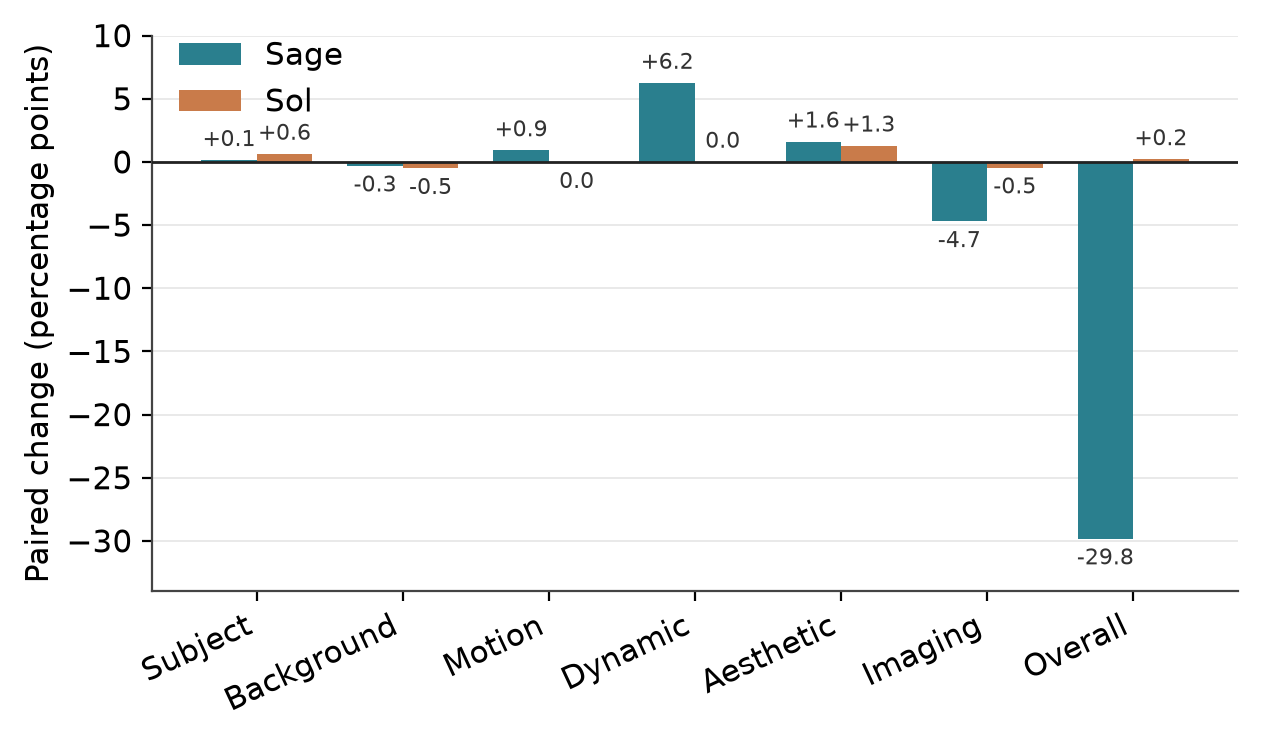
\includegraphics[width=0.85\linewidth]{assets/images/blog/miniacc/chart-quality-deltas.png}
\caption{The same deltas as a chart. Sage's damage concentrates in overall consistency and imaging, and it is consistent across clips, not one outlier.}\label{fig:qualitydeltas}
\end{figure}

Sage's cost is systematic. Overall consistency, which measures whether the video matches the prompt's meaning, dropped on every eligible clip. Imaging quality, a sharpness-and-artifacts score, dropped on 14 of 16 clips. One plausible explanation is that 8-bit attention stacked on 8-bit weights nudges the distilled model off the trajectory it was trained for, but we have not proven that mechanism. Sol, by contrast, is quality-neutral and simply slower, so there is no reason to adopt it. Our default ships with Sage because the speed matters for our use, and the fidelity-first configuration (AdaLN and INT8 without Sage) is one flag away for anyone who would rather keep baseline-level quality at 2.19$\times$.

Finally, here is what all of this looks like. Both clips use the same prompt, \emph{``A person is squat''} (VBench prompt 0195, human action), and the same seed.

\textbf{Baseline serving:}

\begin{figure}[ht]
\centering
\includegraphics[width=0.75\linewidth]{assets/images/blog/miniacc/demo-baseline.gif}
\caption{Baseline serving. Prompt: ``A person is squat''.}
\end{figure}

\textbf{Integrated pipeline:}

\begin{figure}[ht]
\centering
\includegraphics[width=0.75\linewidth]{assets/images/blog/miniacc/demo-pipeline.gif}
\caption{The integrated pipeline. Same prompt and seed.}
\end{figure}

\section{Limitations and what we would do next}

There are several honest caveats. Speed numbers come from single requests on one GPU, so treat them as indicative rather than universal. The quality study is solid on its own scale, but 16 clips and 4 overall-consistency clips are still small samples, and the Sage cost would benefit from a bigger sweep before anyone ships this. We assessed video quality only. The audio track is validated for presence and format but never scored, because we know no good paired metric for generated audio. For scoring we pinned one specific VBench revision and hash-verified all seven of its scorer files before every run, so the scoring code is bit-for-bit reproducible. We did not run or verify VBench-2, so our numbers are not comparable to it. Nothing in principle stops a future pass from pinning and verifying VBench-2 the same way; we simply have not done that work.

The most interesting direction is one we could not touch here, because it needs real training compute. Right now the 8-bit pieces are approximations bolted onto a model distilled for 16-bit arithmetic. With post-training resources, one could distil the model \emph{into} the fast recipe, teaching it to expect 8-bit weights and 8-bit attention rather than tolerate them. That is the standard way to recover the quality cost, and it is also the only honest route we see to making sparse attention competitive: train the sparsity in rather than bolt it on.

The code for the integrated pipeline, including the measured configurations and the demo clips, is on GitHub at \href{https://github.com/TY-Yang3015/MiniAcc}{TY-Yang3015/MiniAcc}.
